
% ==================================================
%	Einleitung
% ==================================================

\section{Einleitung}
\label{sec:einleitung}

Wird in einem Ionenkristall aus einwertigen Ionen ein zweiwertiges Ion
eingebaut, so werden in dem Kristall permanente elektrische Dipole erzeugt.
Mit dem Einbau des zweiwertigen Ions ensteht auch immer eine Leerstelle im
Kristall.
Die Richtung des Dipols weist dabei von der Position des zweiwertigen Ions
zur Leerstelle. In Abbildung \ref{fig:kristall} ist ein Dipol in einem
CsJ-Kristall schemenhaft dargestellt.
%
\begin{figure}[htpb]
	\centering
	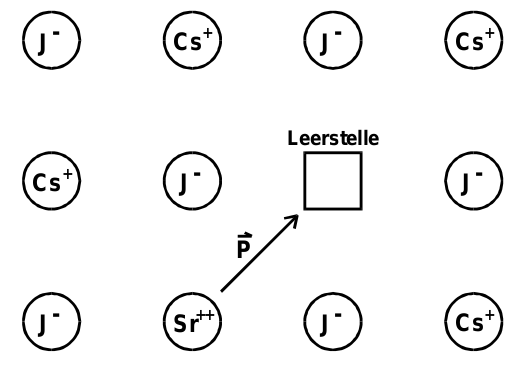
\includegraphics[scale=0.3]{bilder/kristall.png}
	\caption{Darstellung eines Dipols in einem CsJ-Kristalls. \cite{AP}}
	\label{fig:kristall}
\end{figure}
%
Das Fremdatom und die Leerstelle können sich nur auf diskreten Gitterplätzen
aufhalten. Bei Temperaturen unter \SI{500}{\celsius} können sich überwiegend
nur die Leerstellen im Gitter bewegen, womit sich die Richtung des Dipols nur
durch Diffusion der Leerstellen ändern kann. Damit sich die Leerstellen aber
überhaupt bewegen können, muss eine Potentialschwelle, welche durch die
räumlich periodische Anordnung der Gitteratome entsteht, überwunden werden.
Die Energie, die dazu notwendig ist wird als \emph{Aktivierungsenergie} $W$
bezeichnet. Die Gesamtheit der Dipole unterliegt dabei der Boltzman-Statistik.
Die mittlere Zeit zwischen einer Umorientierung des Dipols wird als
\emph{Relaxationszeit} bezeichnet. Sie ist proportional zur Boltzman-Statistik
und lässt sich in Abhängigkeit der Temperatur $T$ durch
%
\begin{equation}
	\tau(T) = \tau_0 \exp(\frac{W}{\kB T})
	\label{eq:relaxationszeit}
\end{equation}
%
ausdrücken.
Dabei ist $\tau_0$ die charakteristische Relaxationszeit und $\kB$ die
Boltzman-Konstante.

\paragraph{Ziel}
\label{par:ziel}

Ziel des Versuches ist es nun die Aktivierungsenergie $W$ und
die charakteristische Relaxationszeit $\tau_0$ für einen KBr Kristall
zu bestimmen.
